\documentclass[12pt]{article}
\input{preamble}

\pagestyle{fancy}
\fancyhf{}

\rhead{Nørre Gymnasium\\
1.m
}


%Husk at rette modul og dato!
\lhead{Matematik B\\
Diverse	
}
\chead{15. maj 2024
}

\cfoot{Side \thepage \hspace{1pt} af \pageref{LastPage}}

\begin{document}

%Udfyld afsnit herunder og lav til egen Latex-fil

%Kopier følgende til overskrift:

%\begin{center}
%\Huge
%Aflevering 1
%\end{center}
%\section*{Opgave 1}
%\stepcounter{section}
%Overskrift

\begin{center}
\Huge
Forberedelse til årsprøve
\end{center}

\section*{Uden hjælpemidler}
\subsection*{Opgave 1}
En eksponentialfunktion $f$ er givet ved
	\begin{align*}
		f(x) = 1.3\cdot 0.97^x.
	\end{align*}
	Bestem fremskrivningsfaktoren og vækstraten for $f$. Afgør desuden hvor mange procent $f$ stiger/falder med, hvis $x$ øges med 1.

\subsection*{Opgave 2}
Bestem forskriften for den eksponentialfunktion, der går gennem punkterne $(1,3)$ og $(3,27)$.

\subsection*{Opgave 3}
Bestem følgende
\begin{align*}
	&1) \  \log_{10}(1000)      &2) \  \log_5(25)       \\
	&3) \  \log_2(16)       &4) \ \log_3(9)         \\
\end{align*}

\newpage

\subsection*{Opgave 4}

Aflæs fordoblings/halveringskonstanten for følgende eksponentialfunktioner.
\begin{center}
\resizebox{0.45\textwidth}{!}{
	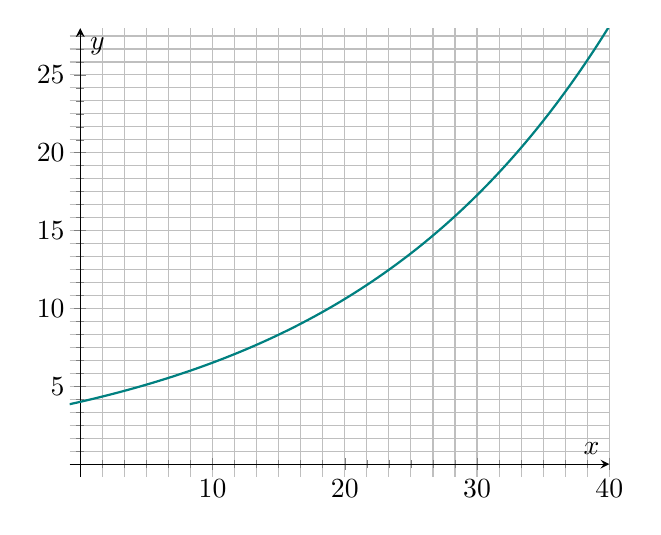
\begin{tikzpicture}
		\begin{axis}[
		axis lines = center,
		xmin = -0.8, xmax = 40,
		ymin = -0.8,ymax = 28,
		grid = both,
		minor tick num = 5,
		xlabel = $x$, ylabel = $y$,
		]
			\addplot[thick, samples = 1000, color = teal, domain = -0.8:40] {4*1.05^x};
		\end{axis}
	\end{tikzpicture}	
}	
\resizebox{0.45\textwidth}{!}{
	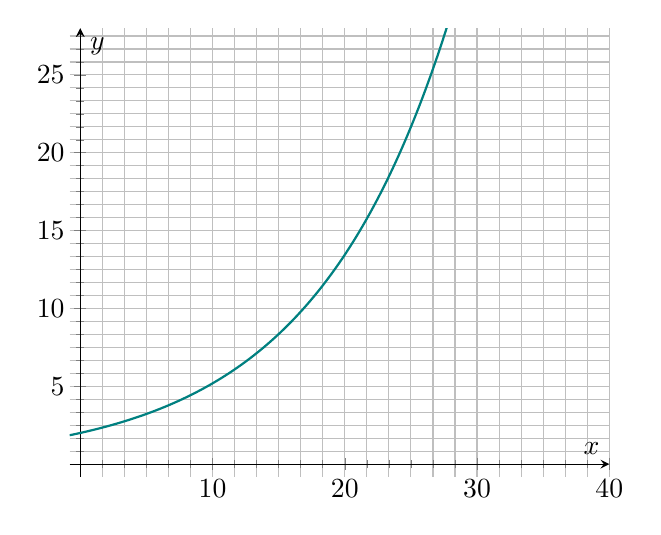
\begin{tikzpicture}
		\begin{axis}[
		axis lines = center,
		xmin = -0.8, xmax = 40,
		ymin = -0.8,ymax = 28,
		grid = both,
		minor tick num = 5,
		xlabel = $x$, ylabel = $y$
		]
			\addplot[thick, samples = 1000, color = teal, domain = -0.8:40] {2*1.1^x};
		\end{axis}
	\end{tikzpicture}
}
\resizebox{0.45\textwidth}{!}{
	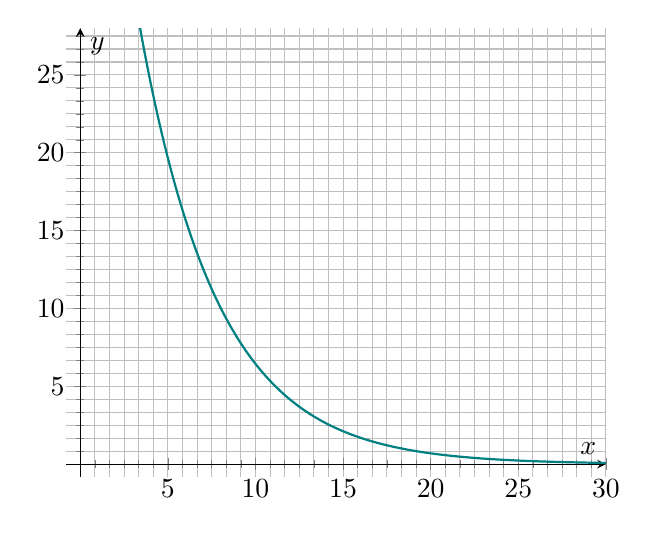
\begin{tikzpicture}
		\begin{axis}[
		axis lines = center,
		xmin = -0.8, xmax = 30,
		ymin = -0.8,ymax = 28,
		grid = both,
		minor tick num = 5,
		xlabel = $x$, ylabel = $y$
		]
			\addplot[thick, samples = 1000, color = teal, domain = -0.8:40] {60*0.8^x};
		\end{axis}
	\end{tikzpicture}
}
\resizebox{0.45\textwidth}{!}{
	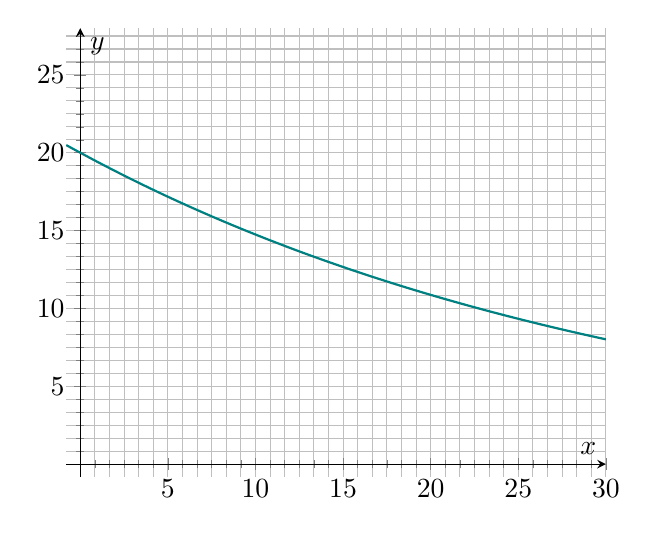
\begin{tikzpicture}
		\begin{axis}[
		axis lines = center,
		xmin = -0.8, xmax = 30,
		ymin = -0.8,ymax = 28,
		grid = both,
		minor tick num = 5,
		xlabel = $x$, ylabel = $y$
		]
			\addplot[thick, samples = 1000, color = teal, domain = -0.8:40] {20*0.97^x};
		\end{axis}
	\end{tikzpicture}
}
\end{center}

\newpage
\subsection*{Opgave 5}

På Figur \ref{fig:opgavegrafer} kan graferne for de to potensfunktioner $f$ og $g$ ses. 
\begin{figure}[H]
	\center
	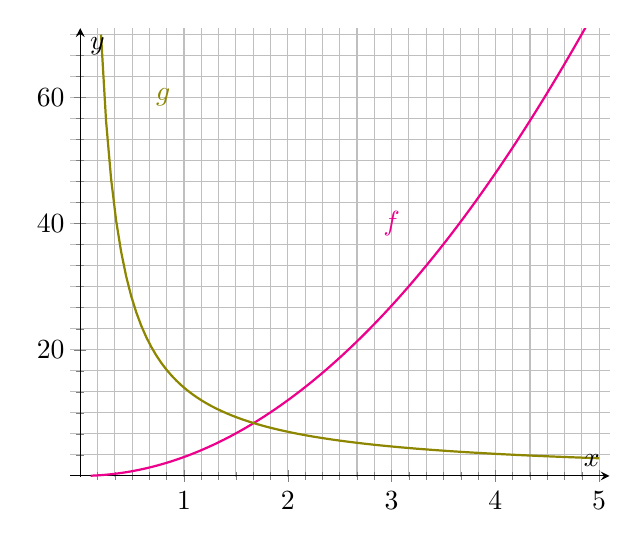
\begin{tikzpicture}
		\begin{axis}[
		axis lines = middle, 
		xmin = -0.1, xmax = 5.1,
		ymin = -0.1, ymax = 71,
		xlabel = $x$, ylabel = $y$, 
		grid = both, minor tick num = 5]
			\addplot[color = magenta, thick, domain = 0.1:5, samples = 100] {3*x^2};		
			\addplot[color = olive, thick, domain = 0.2:5, samples = 100] {14*x^(-1)};
			\node[color = olive] at (axis cs: 0.8,60) {$g$};
			\node[color = magenta] at (axis cs: 3,40) {$f$};
		\end{axis}
	\end{tikzpicture}
	\caption{Grafer for to potensfunktioner $f$ og $g$.}
	\label{fig:opgavegrafer}
\end{figure}
Brug Figur \ref{fig:opgavegrafer} til at løse følgende opgaver.
\begin{enumerate}[label=\roman*)]
	\item Bestem $f(2)$.
	\item Bestem $g(4)$.
	\item Løs ligningen $g(x) = 44$.
	\item Løs ligningen $f(x) = 30$.
	\item Løs ligningen $f(x) = g(x)$.
\end{enumerate}

\newpage
\subsection*{Opgave 6}

Tre potensfunktioner $f$, $g$ og $h$ er givet ved
\begin{align*}
	f(x) &= 3\cdot x ^2\\
	g(x) &= 5\cdot x^{0.7}\\
	h(x) &= 4\cdot x^{-0.8}\\
\end{align*}
Deres grafer er givet på Figur \ref{fig:potensgrafer}.
\begin{figure}[H]
	\centering
	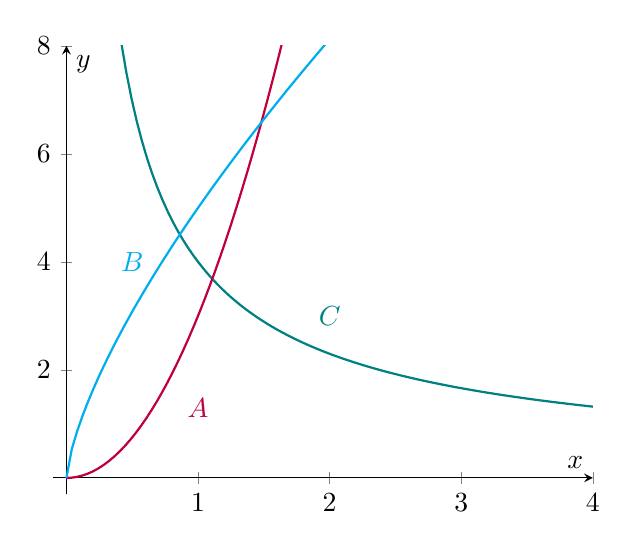
\begin{tikzpicture}
		\begin{axis}
			[axis lines = center, 
			xmin = -0.1, xmax = 4, 
			ymin = -0.3, ymax = 8,
			xlabel = $x$, ylabel = $y$]
			\addplot[color = teal, thick, domain = 0.1:4, samples = 100] {4*x^(-0.8)};
			\addplot[color = purple, thick, domain = 0.0:4, samples = 100] {3*x^(2)};
			\addplot[color = cyan, thick, domain = 0.0:4, samples = 100] {5*x^(0.7)};
			\node[color = purple] at (axis cs: 1,1.3) {$A$};
			\node[color = cyan] at (axis cs: 0.5,4) {$B$};
			\node[color = teal] at (axis cs: 2,3) {$C$};
		\end{axis}
	\end{tikzpicture}
	\caption{Graferne for de tre potensfunktioner $f$, $g$ og $h$.}
	\label{fig:potensgrafer}
\end{figure}

\begin{enumerate}[label=\roman*)]
	\item Afgør hvilke af graferne $A$, $B$ og $C$ der passer med funktionerne $f$, $g$ og $h$.
\end{enumerate}

\subsection*{Opgave 7}

For $f(x) = x^2$ og $g(x)=2x+3$ løs ligningen
\begin{align*}
f(g(x)) = 0.
\end{align*}

\subsection*{Opgave 8}

En stykvist defineret funktion $f$ er givet ved
\begin{align*}
	f(x) = 
	\begin{cases}
		x^2, \ &\textnormal{ hvis } x \geq 0,\\
		-x^2, \ &\textnormal{ hvis } x < 0.
	\end{cases}
\end{align*}
\begin{enumerate}[label=\roman*)]
	\item Bestem $f(3).$
	\item Bestem $f(-4).$
	\item Løs ligningen $f(x) = -64$.
\end{enumerate}

\subsection*{Opgave 9}
For parablen i Figur \ref{fig:andenpolys}
\begin{enumerate}[label=\roman*)]
\item Bestem fortegnet på koefficienterne $a$ og $b$. 
\item Bestem $c$.
\item Bestem fortegnet på diskriminanten $d$.
\end{enumerate}
\begin{figure}[H]
\centering

\begin{tikzpicture}
\begin{axis}
[
	axis lines = middle,
	xmin = -3, xmax = 3, ymin = -2, ymax = 4
 ]
\addplot[thick, samples = 100, color = teal] {-x^2-x+3};
\end{axis}
\end{tikzpicture}


\caption{Parabel}
\label{fig:andenpolys}
\end{figure}

\subsection*{Opgave 10}

Løs ligningen
\begin{align*}
	x^2-3x+2 = 0
\end{align*}

\subsection*{Opgave 11}
Fire punkter er givet ved $A(4,2)$, $B(2,-1)$, $C(-5,-3)$ og $D(9,7)$.
\begin{enumerate}[label=\roman*)]
	\item Bestem koordinaterne til vektorerne $\vv{BA}$, $\vv{CD}$, $\vv{DB}$, $\vv{AC}$ og $\vv{BC}$.
	\item Udregn $\vv{BA} + \vv{CD}$ og $\vv{AC} - \vv{BC}$.
	\item Bestem $\vv{DB}\cdot \vv{BA}$.
	\item Bestem arealet af parallelogrammet udspændt af vektorerne $\vv{CD}$ og $\vv{BC}$.
\end{enumerate}

\subsection*{Opgave 12}
På følgende figur er fire vektorer givet
\begin{center}
	\begin{tikzpicture}
		\begin{axis}[
			axis lines = center, 
			xmin = -3, xmax = 7, 
			ymin = -3, ymax = 7, 
			x = 1.3cm, y = 1.3cm,
			grid,
			xlabel = $x$, ylabel = $y$
		]
			\draw[-{Stealth[scale=1.5]}, thick, color = teal] (axis cs: -2,-2) -- (axis cs: 0,5) node[midway, xshift = -7pt, yshift = 7pt] {$\vv{u}$};
			\draw[-{Stealth[scale=1.5]}, thick, color = teal] (axis cs: 0,6) -- (axis cs: 6,4) node[midway, xshift = 7pt, yshift = 7pt] {$\vv{v}$};
			\draw[-{Stealth[scale=1.5]}, thick, color = teal] (axis cs: 3,3) -- (axis cs: 1,2) node[midway, xshift = -7pt, yshift = 7pt] {$\vv{a}$};
			\draw[-{Stealth[scale=1.5]}, thick, color = teal] (axis cs: 3,3) -- (axis cs: 5,1) node[midway, xshift = 7pt, yshift = 7pt] {$\vv{b}$};
			\fill[olive,nearly transparent] (axis cs: 3,3) -- (axis cs: 5,1) -- (axis cs:3,0) -- (axis cs: 1,2) -- cycle;
		\end{axis}
	\end{tikzpicture}
\end{center}
\begin{enumerate}[label=\roman*)]
	\item Afgør, om vektorerne $\vv{u}$ og $\vv{v}$ er orthogonale.
	\item Bestem arealet af det farvede område.
	\item Vis, at $\vv{u}$ og $\vv{v}$ ikke er parallelle. 
\end{enumerate}



\section*{Med Hjælpemidler}

\subsection*{Opgave 1}

Vi har efter 3 år 6750kr på en konto og efter 7 år 7433kr på samme konto. Beløbet på kontoen kan beskrives ved eksponentiel vækst.
\begin{enumerate}[label=\roman*)]
	\item Bestem den eksponentialfunktion, der beskriver beløbet på kontoen efter $x$ år.
	\item Afgør, hvornår meget der står på kontoen efter 12 år.
	\item Hvornår står der 10.000kr på kontoen?
\end{enumerate}

\subsection*{Opgave 2}

I \href{https://github.com/ChristianJLex/TeachingNotes/raw/master/2022-2023/Data%20og%20lign/Befolkningsdata.xlsx}{\color{blue!60} dette datasæt} fremgår sammenhængen mellem antallet af personer i en by (i tusinde) fra år 1900 til år 2000.

\begin{enumerate}[label=\roman*)]
	\item Anvend eksponentiel regression på datasættet, der beskriver antallet af personer i byen.
	\item Brug din eksponentialregression til at bestemme antallet af personer, der vil være i år 2010 ifølge modellen.
	\item Afgør, hvornår der vil være 150.000 personer i byen ifølge modellen. 
\end{enumerate}

\subsection*{Opgave 3}
Bestem enten fordoblings eller halveringskonstanten for følgende eksponentialfunktioner
\begin{align*}
	&1) \ f_1(x) = 0.5\cdot 2^x   &&2) \ f_2(x)=2\cdot 0.5^x  
\end{align*}


\subsection*{Opgave 4}

I \href{https://github.com/ChristianJLex/TeachingNotes/raw/master/2023-2024/Data%20og%20lign/H%C3%B8jdeV%C3%A6gt.xlsx}{\color{blue!60} dette datasæt} fremgår højde og vægt for 30 personer. Det antages, at sammenhængen mellem højde og vægt kan beskrives af en sammenhæng af typen
\begin{align*}
	f(x) = b \cdot x^a.
\end{align*}

\begin{enumerate}[label=\roman*)]
	\item Lav regression på datasættet.
	\item Brug regressionen til at afgøre, hvad en person på 210 cm vil veje
	\item Hvor høj vil en person være, hvis personen vejer 35 kg?
\end{enumerate}

\subsection*{Opgave 5}
På Figur \ref{fig:potensopg} kan grafen for en potensfunktion $f$ ses. 
\begin{figure}[H]
	\centering
	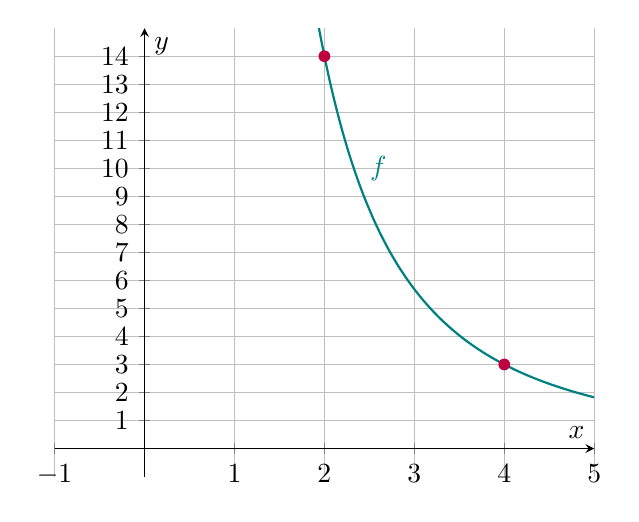
\begin{tikzpicture}
		\begin{axis}[
			axis lines = middle, 
			xmin = -1, xmax = 5,
			ymin = -1, ymax = 15,
			grid = both,
			ytick = {1,2,...,14},
			xlabel = {$x$},
			ylabel = {$y$}
			]
			\addplot[thick, color = teal, samples = 200, domain = 0.4:5]
			{65.333*x^(-2.2224)};
			\node[circle, fill, inner sep = 1.5pt, color = purple] at (axis cs:2,14){};
			\node[circle, fill, inner sep = 1.5pt, color = purple] at (axis cs:4,3){};
			\node[color = teal] at (axis cs:2.6,10) {$f$};
		\end{axis}
	\end{tikzpicture}
	\caption{Graf for potensfunktion $f$.}
	\label{fig:potensopg}
\end{figure}

\begin{enumerate}[label=\roman*)]
	\item Bestem en forskrift for $f$ ved at bruge topunnktsformlen for potensfunktioner
	\item Bestem $f(3)$ og undersøg, om dette passer med Figur \ref{fig:potensopg}.
	\item Løs ligningen $f(x) = 12$.
\end{enumerate}


\subsection*{Opgave 6}
	Et datasæt er givet \href{https://github.com/ChristianJLex/TeachingNotes/raw/master/2023-2024/Data og lign/poly_opgave1.xlsx}{\color{blue!60} her}.
	\begin{enumerate}[label=\roman*)]
		\item Brug residualplots til at bestemme den mindste polynomielle grads regression, 
		der beskriver datasættet godt. 
		\item Lav polynomiel regression med den grad, du har bestemt i i) og bestem 
		forskriften for det polynomium, der beskriver datasættet.
		\item Brug forskriften til at bestemme $f(4)$.
		\item Brug Maple til at finde rødderne for $f$.
	\end{enumerate}

\subsection*{Opgave 7}

To vektorer $\vv{a}$ og $\vv{b}$ er givet ved
\begin{align*}
	&\vv{a} =	
	\begin{pmatrix}
		x^2 \\ -2
	\end{pmatrix}
	&
	&\textnormal{og}
	&
	&\vv{b} =
	\begin{pmatrix}
		1 \\ x+4
	\end{pmatrix}
\end{align*}

\begin{enumerate}[label=\roman*)]
	\item Bestem prikproduktet mellem $\vv{a}$ og $\vv{b}$, hvis $x = 6$.
	\item Bestem de værdier for $x$, der gør $\vv{a}$ og $\vv{b}$ orthogonale. 
\end{enumerate}




\end{document}
